\chapter{Implementation}\label{sec:implementation}


This section describes the reference implementation for the conceptual framework in Chapter \ref{sec:concept}.
First, the general architecture is explained.
Various components and interaction techniques of the geographical visualization are detailed.
The integration of the geographical visualization in the existing \visan{} is shown.
The connection of the conceptual framework and the implemented framework is examined.

\section{Implemented interactions}

In the course of this thesis the following interactions have been implemented:
\begin{itemize}
  \item
    Select

    \begin{itemize}
      \item
        Highlighting an entity is possible by moving the mouse cursor on a geographic feature in the \gv{} or a block in the \tmap{}.
        The corresponding block or geographic feature will be highlighted respectively.
      \item
        A click on a block in the \tmap{} selects this entity in the \gv{} and vice versa.
      \item
        Holding the control key, multiple clicks on a block in the \tmap{} creates a group of selected entities.
        Corresponding geographic feature or blocks in the \tmap{} or \gv{} are selected as well.
    \end{itemize}

  \item
    Explore

    \begin{itemize}
      \item Selecting a block in the \tmap{} centers the viewpoint in the \gv{} on the corresponding geographic feature.
      \item Selecting a group of blocks in the \tmap{} centers the viewpoint in the \gv{} on the boundaries of all corresponding geographic features.
    \end{itemize}

  \item
    Reconfigure

    \begin{itemize}
      \item
        Choosing a different data set updates the geometries in the \gv{}.
      \item
        Selecting another shape for the \tmap{} (e.g. point instead of polygon geometries) changes the visual representation in the \gv{}.
    \end{itemize}

  % \item
  %   \emph{Filter}: The user double-clicks on a region in a geographical map and the \tmap{} will be based on data of only that region.
\end{itemize}
\todo[inline]{If we still have time, add filter interaction here}

\section{Overview of the Layout}

Figure~\ref{fig:implementation:layout} shows the layout of the different views from the user perspective.
The \tmap{} is on the left while the \gv{} is on the right.
Some additional views like the message log and a form to manually change the highlighted item are visible as well.

The figure shows a screenshot of the \visan{}, currently visualizing the data set ``Wahlkreise''.
The \tmap{} is tiled based on unemployment rate and the colour is based on the percentage of high-school graduates.
Currently the district ``Magdeburg'' is selected in the \gv{} with an unusually high percentage of graduates for its unemployment rate.

\begin{figure}[ht]
  \centering
  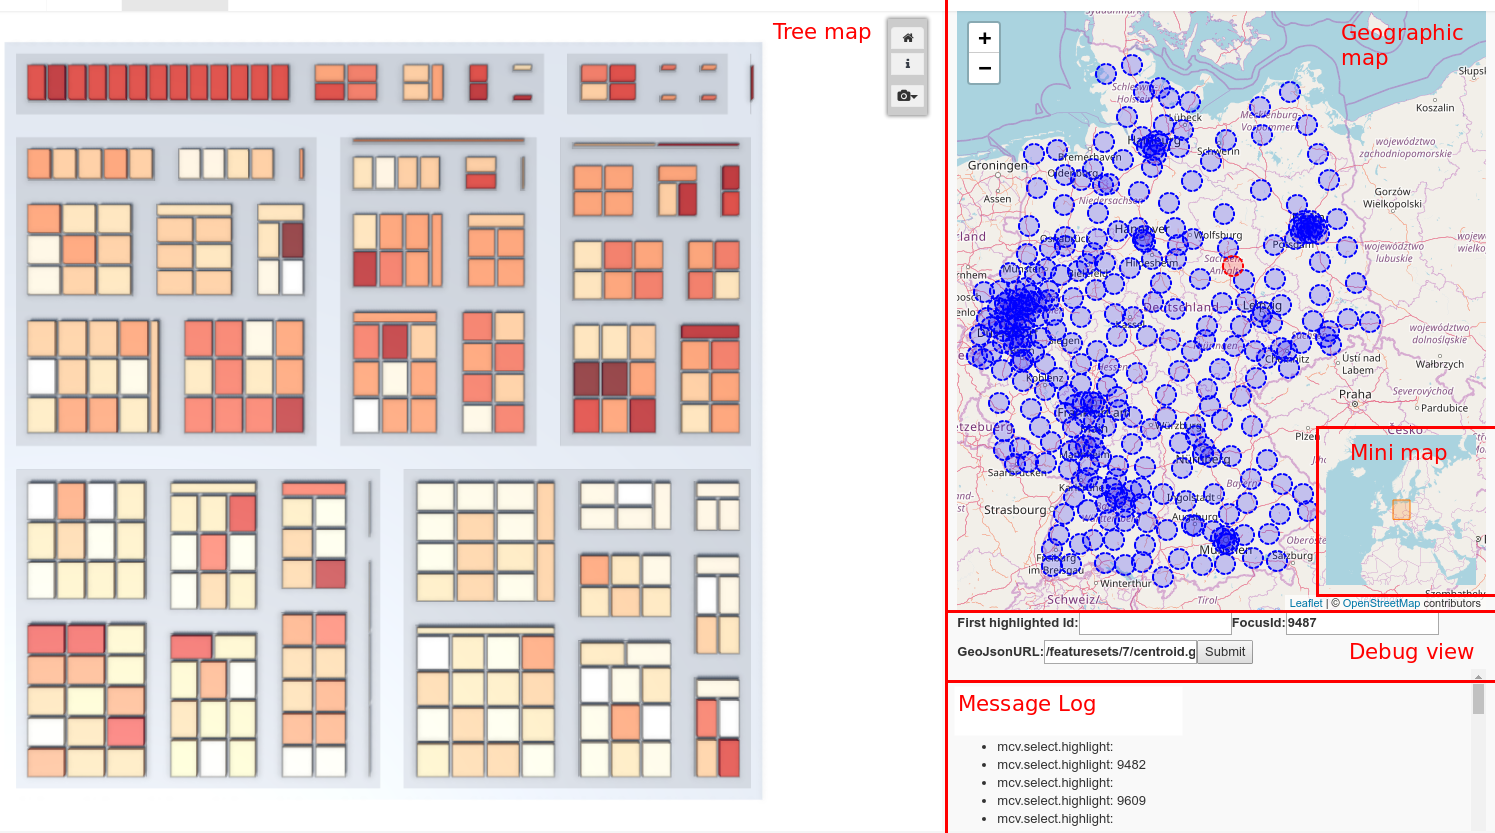
\includegraphics[width=\textwidth]{figures/implementation/Layout}
  \caption{%
    This Figure shows the layout of the \cmv{}, red lines indicate the borders of different views.
  }\label{fig:implementation:layout}
\end{figure}


\section{Architecture}
Figure~\ref{fig:implementation:architecture} shows classes and their relations in the \cmv{} implementation of \tmap{} and \gv{}.

\attr{UAController} is a class of the existing \visan{} and controls the rendering of the \tmap{}.
The rendering of the geographical visualization is controlled by the class \attr{MapComponent}.

Classes with a \attr{render} method are views and can be rendered in place of a node inside the DOM tree.
Those views are implemented as React components and therefore have a native update mechanism, i.e.\ they get automatically re-rendered if their internal state changes.
Except of a dependency to a \attr{MultiviewCoordinator}, they are dependency free, which makes those classes easy to test.

Additionally, there are two other views, \attr{DebugView} and \attr{MessageLog}.
These views record interactions at runtime and can trigger and simulate an interaction.

State and changes shared between views are controlled by the \attr{MultiviewCoordinator}.
Every view has a reference to \attr{MultiviewCoordinator} in order to subscribe to interactions.
The \attr{MultiviewCoordinator} itself does not have a visual representation.

\begin{figure}[ht]
  \centering
  \caption{%
    Architecture of components.
    Every class with a \attr{render} method is a React component.
    \attr{MultiviewCoordinator} is used to coordinate \tmap{} and \gv{} as well as to load geometry data.
  }\label{fig:implementation:architecture}
  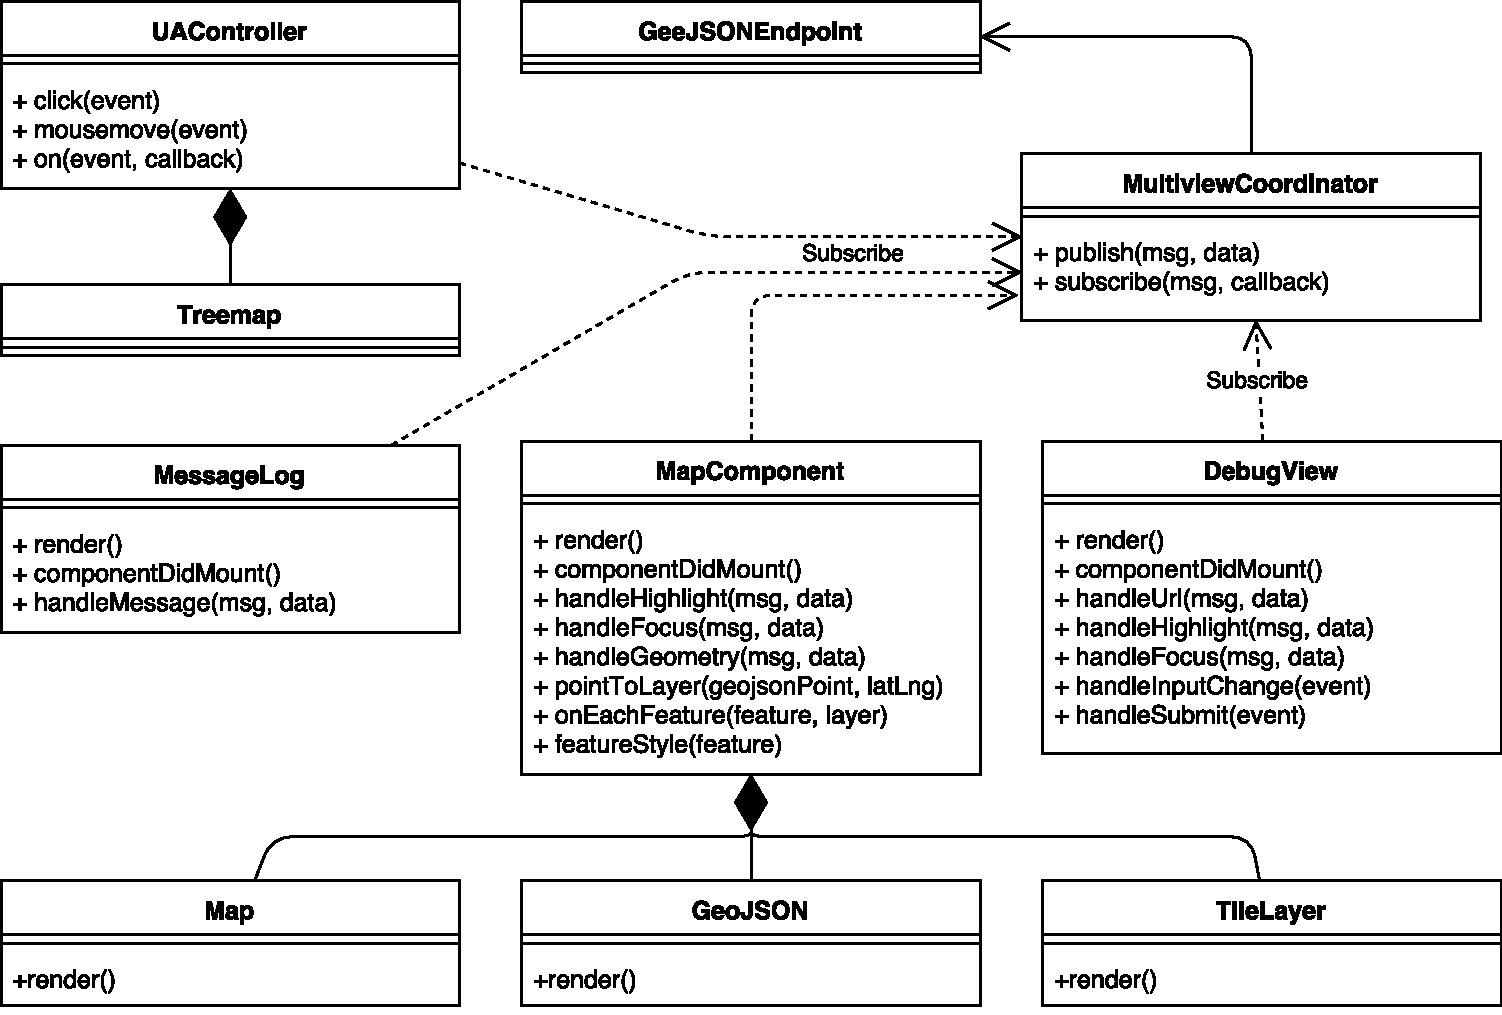
\includegraphics[width=\textwidth]{figures/implementation/Architecture.pdf}
\end{figure}


\section{Adding the views to the DOM}

Adding the \gv{} to the DOM is straightforward.
Listing~\ref{lst:implementation:dom} shows an example how to use React's low-level API to render components inside the DOM.
It uses an id \attr{multiview-map-component} to reference a particular node in the HTML document in Listing~\ref{lst:implementation:dom-html} on line 3.
On lines 4 to 6 you can see the required JavaScript imports, i.e.\ two imports required by React and the compiled JavaScript application, which is called \attr{example.js}.

\lstinputlisting[
  label={lst:implementation:dom},
  lastline=12,
  caption={
    Example application written in TypeScript.
    Views can be added to the DOM individually.
    The implementation exposes convenient TypeScript declarations, here \attr{MultiviewCoordinator} and \attr{MapComponent} are imported.
  }
]{listings/implementation/dom.tsx}

\lstinputlisting[
  label={lst:implementation:dom-html},
  caption={
    This short HTML document shows how to render Views at a certain node inside the DOM.
    The id multiview-map-component is used as anchor.
  },
  language=HTML
]{listings/implementation/dom.html}

The reference implementation of the conceptual framework is written in \attr{TypeScript}\footnotemark.
The implementation exports typescript declaration and you can see an import of the classes \attr{MapComponent} and \attr{MultiviewCoordinator} on lines 1 to 3 in Listing~\ref{lst:implementation:dom}.
\footnotetext{
  TypeScript is a typed superset of JavaScript that compiles to plain JavaScript.
  It provides optional static typing, classes and interfaces and helps to reduce errors by raising type errors at compile time.
}





Event handlers just have to publish an interaction, if the view is subscribed to the same interaction, it will automatically re-render.

\section{MultiviewCoordinator}


The \attr{MultiviewCoordinator} uses the \attr{publish-subscribe} pattern for coordination and works as a broker for interactions across \cmvs{}.
In order to accomplish that it uses the JavaScript library \attr{PubSubJS} which is an topic-based, asynchronous implementation of the pattern.

Geometry data is exchanged with \attr{GeoJSON}\footnotemark as data format.
\footnotetext{
  GeoJSON is a format for encoding a variety of geographic data structures~\cite{GeoJSON2017}.
  Based on JSON, it can represent simple geographic features like points, lines and areas and reserves a properties object for non-spatial attributes.
}

As the central part of the software, the \attr{MultiviewCoordinator} is also used for certain performance optimizations.
The optimizations affect how often the geometries are reloaded, i.e.\ it reduces the number of requests to the \attr{GeoJSON} endpoint.


\lstinputlisting[
  label={lst:implementation:multiviewController},
  caption={The \attr{multiviewController} avoids unnecessary requests to reload geometries}
]{listings/implementation/multiviewController.tsx}

As shown in Listing~\ref{lst:implementation:multiviewController}, the geometries depend on a change of the \attr{url} of the geometries.
A change of the \attr{url} will automatically trigger an interaction of type \attr{reconfigure} to reload geometries.

An example of these geometries can be seen in listing~\ref{lst:geojson:example}.
For convenience, the file includes the aggregated data in the \attr{properties} of each feature.
In this case the colors the shapes of the \tmap{} are based on the value of \attr{user_count_normalized}.
Each feature comes with a unique \attr{id} which is published when a user interacts with the feature.

\lstinputlisting[
  label={lst:geojson:example},
  caption={A truncated example of a user distribution across German federal states}
]{listings/implementation/example.geojson}

\section{Software patterns}\label{sec:implementation:patterns}
Figure~\ref{fig:implementation:sequence-diagram} shows how \cmvs{} can be automatically updated even if the environment lacks a native update-mechanism.

\begin{figure}[ht]
  \centering
  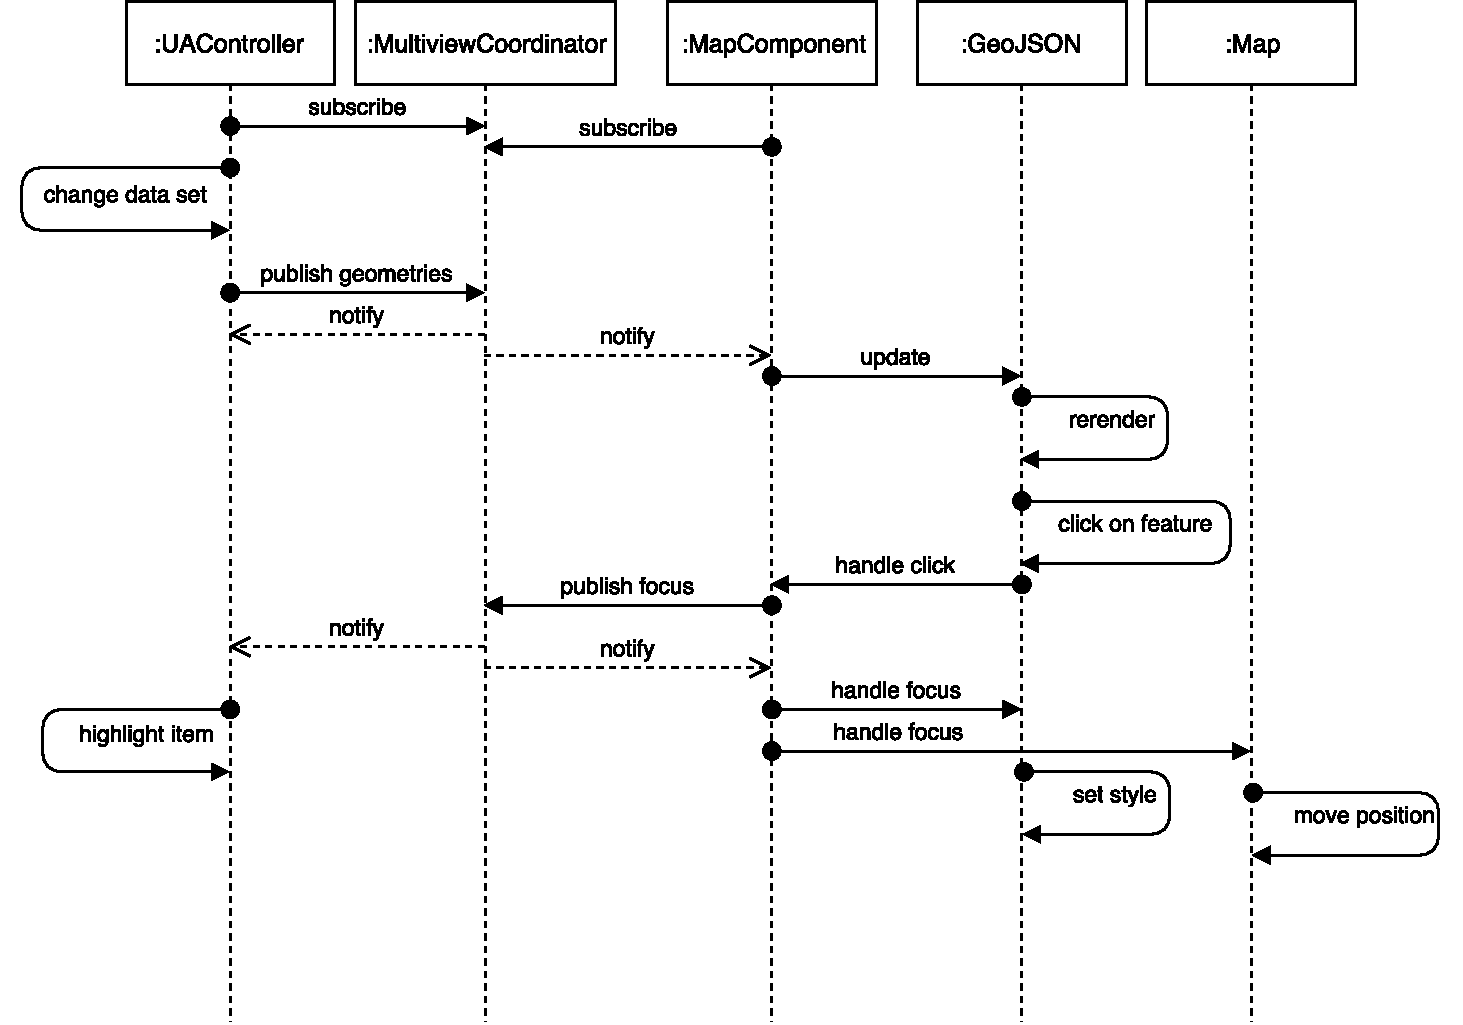
\includegraphics[width=\textwidth]{figures/implementation/SequenceDiagram}
  \caption{%
    The sequence diagram shows the notification of different components.
  The user first chooses a feature set and clicks on a polygon in the \gv{}.
  }\label{fig:implementation:sequence-diagram}
\end{figure}


\textbf{The Observer pattern} allows multiple \emph{observers} to react to changes of an observed state.
In our case, the observed state is the \attr{MultiviewCoordinator}.
Any change to the \attr{MultiviewCoordinator} will subsequently be broadcasted to all connected views.


\textbf{Publisher subscriber}
In our particular case we apply a special form of the observer pattern, the so called ``Publish-subscribe'' pattern\cite{Eugster2003}.
Publish-subscribe is a messaging pattern which is widely used in message queues.
In this scenario, senders of messages simply categorize their messages which will be consumed by subscribers of the category.
The scenario has very low coupling, publishers do not even need to know the existence of subscribers.

\textbf{Component pattern}
State-of-the-art JavaScript component frameworks like ReactJS and EmberJS follow the component pattern for the architecture of a single page web application.
The component pattern imposes a hierarchical structure on a website.
Each component is responsible for a task and may contain other components.
The components are joined at the root node of the page.

This pattern is very applicable to \cmvs{}.
The different views of \cmvs{} share state, i.e.\ the feature, that is currently highlighted or the applied filter on the data.
So the views are components and their closest common ancestor is the \cmv{} itself, controlling state and passing user interaction down to it's children.

\textbf{Actions up --- Data down}

Version 2.0 of Ember introduced a common phrase how to use this pattern effectively: ``Data down, actions up''\cite{Emberigniter2017}
In the domain of \cmvs{} actions would mean user interactions, e.g.\ a click on a feature.
The action will notify the controlling \cmv{} component.
Actions may change data, and the changes will be passed to to all dependent views.
These views are then re-rendered.

Examples for the kind of data that might trigger a re-rendering of a view:
\begin{itemize}
  \item
    The selected feature or a list of selected features
  \item
    A list of thresholds for certain features as a filter
\end{itemize}


\section{Map Component}

The geographical visualization is implemented as a \attr{Map} component of the React Leaflet library.
Listing \ref{lst:implementation:render} shows the \attr{render} method of the component.

\lstinputlisting[
  label={lst:implementation:render},
  caption={\attr{render} method of the Map component of the geographical visualization}
]{listings/implementation/render.tsx}

The \attr{render} method is the only required method of a React component.
It will be invoked on the initial rendering of the component of the \attr{DOM} and on every update of the component's properties.
React's templating language ``\attr{JSX}'' allows to nest other child components into the React parent component.
In this case the \attr{Map} component includes a \attr{TileLayer} \attr{GeoJSON} component from the \attr{react-leaflet} library.
This library conveniently provides ``React components for Leaflet maps.''~\cite{ReactLeaflet2017}.

\subsection{GeoJSON Component}

The \attr{GeoJSON} component is provided by the \attr{Map} component with a couple of properties:
It gets a
\begin{enumerate*}[label=(\arabic*)]
  \item
    geojsonURL as well as a
  \item
    geojson as data attribute. Furthermore a couple of callbacks is passed into the child component, including
  \item
    featureStyle,
  \item
    pointToLayer and
  \item
    onEachFeature.
\end{enumerate*}

This way, the parent \attr{Map} component controls the data flow and without a \attr{geojson} object, no polygons are placed on the map.
A changed \attr{geojsonURL} will always update the child component as it is used a \attr{key} on the \attr{GeoJSON} component.
The callbacks passed into the \attr{GeoJSON} component control the visual representation of each polygon and they add event handlers for a mouse click or a mouse move on each polygon.
Listing \ref{lst:implementation:onEachFeature} shows the event handlers added to the map.

\lstinputlisting[
  label={lst:implementation:onEachFeature},
  caption={\attr{onEachFeature} callback, adding handlers for mouse events}
]{listings/implementation/onEachFeature.tsx}

First we cache all layers in the internal state of the \attr{Map} component.
On each \attr{mouseover} event, the \attr{id} of the feature is published as \attr{mcv.select.highlight} interaction.
A \attr{click} event is distinguished if the control key is pressed or not.
In the latter case, the id of the feature is either added or removed from the list of focused ids and then the list of focused ids is published as \attr{mcv.select.focus} interaction.

\lstinputlisting[
  label={lst:implementation:featureStyle},
  caption={\attr{featureStyle} callback, configuring the visual appearance depending on the currently highlighted or focused feature ids}
]{listings/implementation/featureStyle.tsx}

The \attr{featureStyle} in Listing \ref{lst:implementation:featureStyle} method is very straightforward.
If the feature is currently focused, the \attr{fillColor} of the polygon is red, otherwise blue.
Likewise, if the feature is currently highlighted, the polygon has a white, solid stroke.

\lstinputlisting[
  label={lst:implementation:pointToLayer},
  caption={\attr{pointToLayer} callback, if a feature of \attr{GeoJSON} has a point geometry, it will be shown as a circle}
]{listings/implementation/pointToLayer.tsx}

Finally, we configure how to display point geometries in callback \attr{poinToLayer}.
Since normal markers do not have a configurable color and style, we instruct the \attr{GeoJSON} component to render a \attr{CircleMarker} for each point geometry instead.
This way, the same options of \attr{featureStyle} can be applied to both point and area geometries.




